% =====================================================================
\section{Fase de Producción}
\label{sec:des-produccion}

En esta fase de producción se realiza el desarrollo de las funcionalidades 
planteadas en el diseño con React Native. El desarrollo se realizo en iteraciones,
según la planificación. En cada iteración se definieron las historias de usuario y sus criterios
de aceptación. A partir de ellos, se codificaron los procesos diseñados
y se verificó el funcionamiento de cada módulo antes de integrarlo con
los demás componentes de la aplicación.

\subsection{Estructura de directorios}

A continuación, el Código~\ref{lst:estructura} muestra la estructura de la aplicación y una
breve descripción de los directorios más importantes.

\begin{lstlisting}[language={}, numbers=none, caption={Estructura de carpetas del código fuente}, label={lst:estructura}]
coach-app/
  src/
    app/
      (auth)/
      (onboarding)/
      (app)/
        routines/
        machines/
        progress/
    components/
    controllers/
    utils/
    hooks/
    store/
    models/
      entities/
      repositories/
    schemas/
    services/
      firebase/
      wger/
      usda/
      exercisedb/
      ai/
      ar/
      reports/
    config/
    constants/
    types/
    media/
  modules/
    coach-ar/
  assets/
    models/
  android/
  ml/
    detection/
    recognition-yolo/
  functions/
    src/
    test/
  tests/
    security/
  docs/
  .github/
    workflows/
\end{lstlisting} 

\begin{itemize}
    \item \textbf{Carpeta \archivo{src/app/}:} contiene las pantallas de la
    aplicación y la definición de las rutas mediante Expo Router. Incluye el
    diseño raíz, que protege las rutas según el estado de la sesión y del
    perfil, y los grupos de pantallas de acceso (\archivo{(auth)}), de
    configuración inicial (\archivo{(onboarding)}) y de la aplicación
    autenticada (\archivo{(app)}) con su barra de pestañas.
    \item \textbf{Carpeta \archivo{src/components/}:} contiene los
    componentes visuales reutilizables, organizados por módulo (inicio,
    máquinas, rutinas, nutrición, progreso y entrenamiento) y un conjunto de
    componentes comunes de interfaz.
    \item \textbf{Carpeta \archivo{src/controllers/}:} contiene la lógica de
    negocio. Cada controlador conecta las pantallas con los datos: valida la
    información, coordina los repositorios y devuelve a la vista un resultado
    listo para mostrar.
    \item \textbf{Carpeta \archivo{src/utils/}:} contiene las reglas y los
    cálculos que no dependen de la interfaz, como el índice de masa corporal,
    las metas calóricas, el generador de rutinas, las estadísticas de
    entrenamiento y el reporte de progreso.
    \item \textbf{Carpeta \archivo{src/models/}:} contiene las entidades del
    dominio (usuario, máquina, rutina, entrenamiento, registro nutricional y
    progreso físico) y los repositorios, que son los únicos archivos que
    conocen la estructura de las colecciones de Firestore.
    \item \textbf{Carpeta \archivo{src/schemas/}:} contiene los esquemas de
    validación con Zod que verifican los datos antes de guardarlos y al
    recibirlos de servicios externos.
    \item \textbf{Carpeta \archivo{src/services/}:} contiene los archivos que
    se comunican con servicios externos: la conexión con Firebase
    (autenticación, Firestore, Storage, Cloud Functions y App Check), las
    API de wger y de USDA, los modelos de inteligencia artificial, la interfaz
    de realidad aumentada y la generación del reporte en PDF.
    \item \textbf{Carpetas \archivo{src/hooks/} y \archivo{src/store/}:}
    contienen la lógica de las pantallas y las suscripciones en tiempo real a
    Firebase, y el estado global de la sesión, del onboarding y de los avisos
    (Zustand).
    \item \textbf{Carpeta \archivo{modules/coach-ar/}:} contiene el módulo
    nativo escrito en Kotlin que usa ARCore para anclar la ficha de la máquina
    reconocida sobre la imagen de la cámara.
    \item \textbf{Carpeta \archivo{functions/}:} contiene las Cloud Functions
    del servidor (Node.js 22): la búsqueda de alimentos en USDA, el guardado
    de rutinas, el reconocimiento de máquinas con el detector de Ultralytics y
    el control de cuotas de uso. Las claves de los servicios externos se
    guardan solo en el servidor.
    \item \textbf{Carpeta \archivo{ml/}:} contiene los \emph{scripts} en
    Python con los que se entrenaron, evaluaron y exportaron los modelos de
    recomendación de rutinas y de reconocimiento de máquinas, junto con sus
    métricas.
    \item \textbf{Carpeta \archivo{assets/}:} contiene las imágenes necesarias 
    para el proyecto, logo de la app, etc.
    \item \textbf{Carpeta \archivo{tests/security/}:} contiene las pruebas de
    las reglas de seguridad de Firestore y Storage, que se ejecutan con el
    emulador de Firebase.
\end{itemize}

% ---------------------------------------------------------------------
\subsection{Iteración 1: Autenticación, registro y onboarding}
\label{subsec:it1}

\subsubsection{Pantalla de inicio de sesión.}

Esta pantalla permite iniciar sesión con correo electrónico y contraseña
o iniciar sesión con una cuenta registrada o de Google. El controlador de
autenticación delega la gestión de las credenciales a Firebase Authentication.
Al registrar una cuenta con correo electrónico, la aplicación crea el perfil
del usuario en Cloud Firestore. Cuando el usuario inicia sesión con Google,
la aplicación verifica si ya existe un perfil asociado a su cuenta. Si lo
encuentra, conserva los datos registrados. Si es el primer acceso, crea el
perfil correspondiente (Código~\ref{lst:auth-registro}).

\begin{lstlisting}[language=TypeScript, caption={Registro e inicio de sesión con Google en \texttt{AuthController}}, label={lst:auth-registro}]
async registrar(datos: DatosRegistro): Promise<string> {
  const credencial = await createUserWithEmailAndPassword(
    auth, datos.correo, datos.contrasena);
  const uid = credencial.user.uid;
  await crearPerfilUsuario(uid, {
    nombre: datos.nombre, apellidos: datos.apellidos,
    genero: datos.genero, email: datos.correo,
  });
  return uid;
},

async iniciarSesionConGoogle(idToken: string): Promise<UsuarioSesion> {
  const credencial = GoogleAuthProvider.credential(idToken);
  const { user } = await signInWithCredential(auth, credencial);
  await AuthController.asegurarPerfil(user.uid, {
    nombre: user.displayName, email: user.email,
  });
  return aUsuarioSesion(user);
},
\end{lstlisting}

A continuación, se detalla la lógica de integración para la autenticación:
La autenticación comienza cuando el usuario selecciona su cuenta mediante 
Google Sign-In. Si la operación es exitosa, la aplicación obtiene un token 
de identidad (idToken) y lo utiliza para generar una credencial con la 
que inicia sesión en Firebase Authentication. Una vez autenticado el usuario, 
la aplicación comprueba si existe un perfil asociado a su cuenta en Cloud 
Firestore. Si el perfil ya existe, conserva los datos registrados y dirige 
al usuario a la pantalla correspondiente según el estado de su perfil. Si 
es su primer acceso, crea el perfil y lo dirige a la pantalla de configuración 
inicial.

Los formularios se validan con esquemas Zod antes de llamar al controlador:
el registro exige nombre y apellido, un correo válido, una contraseña de al
menos seis caracteres y la coincidencia con su confirmación.

\paragraph{Estado de la sesión.} Un \emph{store} de Zustand mantiene el estado
global. En el diseño raíz, \archivo{useAuthListener} observa la sesión de
Firebase y \archivo{useProfileListener} consulta el perfil en tiempo real.
El acceso a \archivo{(app)} se habilita cuando el perfil contiene objetivo y
nivel; en caso contrario, el usuario pasa al \emph{onboarding}
(Figura~\ref{fig:secuencia-login}).

\begin{figure}[H]
\centering
\begin{tikzpicture}[font=\scriptsize, x=2.45cm, y=0.72cm,
  part/.style={rectangle, draw=black!70, fill=green!8, minimum width=2.0cm,
    minimum height=0.6cm, align=center, font=\tiny\bfseries},
  msg/.style={-{Stealth[length=2mm]}, thick},
  ret/.style={-{Stealth[length=2mm]}, dashed, black!60}]
  \foreach \i/\n in {0/Usuario, 1/Login, 2/AuthController, 3/Firebase Auth, 4/Firestore, 5/Layout raíz} {
    \node[part] (p\i) at (\i,0) {\n};
    \draw[black!40, dashed] (\i,-0.5) -- (\i,-11.2);
  }
  \draw[msg] (0,-1.6) -- node[above]{correo y contraseña} (1,-1.6);
  \node[draw, fill=white, font=\tiny, anchor=west] at (1.05,-2.3) {valida con Zod};
  \draw[msg] (1,-3.4) -- node[above]{iniciarSesion()} (2,-3.4);
  \draw[msg] (2,-4.4) -- node[above]{signInWith...()} (3,-4.4);
  \draw[ret] (3,-5.4) -- node[above]{sesión (uid)} (2,-5.4);
  \draw[ret] (3,-6.6) -- node[above, pos=0.5]{onAuthStateChanged $\rightarrow$ store} (5,-6.6);
  \draw[msg] (5,-7.8) -- node[above]{observar usuarios/\{uid\}} (4,-7.8);
  \draw[ret] (4,-9.0) -- node[above]{perfil} (5,-9.0);
  \node[draw, fill=white, align=left, font=\scriptsize, anchor=north east] at (5.1,-9.5)
    {¿perfil completo?\\sí $\rightarrow$ \texttt{(app)}\\no $\rightarrow$ \texttt{(onboarding)}};
\end{tikzpicture}
\caption{Diagrama de secuencia del inicio de sesión}
\label{fig:secuencia-login}
\fuente{Elaboración propia.}
\end{figure}

\paragraph{Configuración inicial del perfil.} El \emph{onboarding} reúne tres
pasos: elección del objetivo y nivel, registro de datos físicos y selección
del tipo de rutina. Las pantallas comparten un borrador temporal en Zustand;
al finalizar, el controlador guarda los datos en Firestore y habilita el
acceso a la aplicación. La opción de rutina elegida se abre desde el inicio.
Los datos del perfil se utilizan en el generador de rutinas.

A continuación se presentan las \emph{Story Cards} de la primera iteración:
la Tabla~\ref{tab:hu-it1-login} corresponde al inicio de sesión y la
Tabla~\ref{tab:hu-it1-registro}, al registro de usuario y la configuración
de su perfil.

\begin{table}[H]
\centering
\small
\renewcommand{\arraystretch}{1.2}

\subsubsection{Planificación}

\begin{tabularx}{\textwidth}{|Y|Y|Y|}
\hline
\rowcolor{encabezado}
\textbf{Story Card} & \textbf{Nombre del proyecto} & \textbf{Estimación} \\
\hline
01  & CoachApp& 20 horas \\
\hline

\multicolumn{2}{|l|}{\textbf{Nombre.} Inicio de sesión}
& \textbf{Fecha.} 10/03/2026 \\
\hline

\multicolumn{3}{|l|}{\textbf{Descripción}} \\
\hline
\multicolumn{3}{|p{\dimexpr\textwidth-2\tabcolsep-2\arrayrulewidth\relax}|}{%
El usuario puede iniciar sesión con su correo electrónico y contraseña o con
su cuenta de Google. Tras autenticarse, la aplicación consulta su perfil en Cloud Firestore: si está
completo, lo dirige a la pantalla principal; si está incompleto, lo dirige a
la configuración inicial.
} \\
\hline

\multicolumn{3}{|l|}{\textbf{Prueba de aceptación}} \\
\hline

\multicolumn{3}{|p{\dimexpr\textwidth-2\tabcolsep-2\arrayrulewidth\relax}|}{%
El usuario intenta iniciar sesión con Google.
} \\
\hline

\multicolumn{3}{|p{\dimexpr\textwidth-2\tabcolsep-2\arrayrulewidth\relax}|}{%
El usuario intenta iniciar sesion con correo y contraseña.
} \\
\hline

\multicolumn{3}{|p{\dimexpr\textwidth-2\tabcolsep-2\arrayrulewidth\relax}|}{%
Iniciar sesión con un perfil incompleto y verificar que la aplicación
dirige al usuario a la configuración inicial y restringe el acceso a
las pantallas principales hasta completar el perfil.
} \\
\hline

\multicolumn{2}{|l|}{\textbf{Excepciones}}
& \textbf{Riesgo.} Alto \\
\hline

\multicolumn{3}{|p{\dimexpr\textwidth-2\tabcolsep-2\arrayrulewidth\relax}|}{%
Si el correo o la contraseña son incorrectos, o el usuario cancela el
acceso con Google, se muestra el mensaje de error correspondiente y no se
inicia la sesión.
} \\
\hline

\end{tabularx}
\caption{Story Card 01: Inicio de sesión}
\label{tab:hu-it1-login}
\fuente{Elaboración propia.}
\end{table}

\subsubsection{Codificación}

\capturados{login}{Inicio de sesión}{inicio-de-sesion-2}{Inicio de sesion con Google}
  {Pantallas de inicio de sesión con correo y contraseña o Google}{fig:cap-auth}

\subsubsection{Pantalla de registro.}

En esta pantalla el usuario crea una cuenta ingresando su nombre, correo electrónico y
contraseña. Firebase Authentication registra la cuenta y la aplicación
crea el perfil del usuario en Cloud Firestore
(Código~\ref{lst:auth-registro}).

\subsubsection{Pantalla de registro.}

En esta pantalla el usuario crea una cuenta ingresando su nombre, apellido,
correo electrónico y contraseña. El formulario se valida con un esquema Zod:
exige nombre y apellido, un correo válido, una contraseña de al menos seis
caracteres y que coincida con su confirmación. Luego, Firebase Authentication
registra la cuenta y la aplicación crea el perfil del usuario en Cloud
Firestore.

\begin{lstlisting}[language=TypeScript, caption={Validación del formulario y registro en \texttt{AuthController}}, label={lst:registro}]
export const registroFormSchema = z
  .object({
    nombre: z.string().trim().min(1, "Ingresa tu nombre").max(100),
    apellidos: z.string().trim().min(1, "Ingresa tu apellido").max(100),
    correo: z.string().trim().email("Correo electrónico inválido"),
    contrasena: z.string().min(6, "Mínimo 6 caracteres"),
    confirmarContrasena: z.string(),
  })
  .refine((d) => d.contrasena === d.confirmarContrasena, {
    message: "Las contraseñas no coinciden",
    path: ["confirmarContrasena"],
  });

async registrar(datos: DatosRegistro): Promise<string> {
  const credencial = await createUserWithEmailAndPassword(
    auth, datos.correo, datos.contrasena);
  const uid = credencial.user.uid;
  await crearPerfilUsuario(uid, {
    nombre: datos.nombre, apellidos: datos.apellidos,
    genero: datos.genero, email: datos.correo,
  });
  return uid;
},
\end{lstlisting}

\subsubsection{Planificación}

\begin{table}[H]
\centering
\small
\renewcommand{\arraystretch}{1.2}

\begin{tabularx}{\textwidth}{|Y|Y|Y|}
\hline
\rowcolor{encabezado}
\textbf{Story Card} & \textbf{Nombre del proyecto} & \textbf{Estimación} \\
\hline
02 & CoachApp & 20 horas \\
\hline

\multicolumn{2}{|l|}{\textbf{Nombre.} Registro de usuario y configuración del perfil}
& \textbf{Fecha.} 14/03/2026 \\
\hline

\multicolumn{3}{|l|}{\textbf{Descripción}} \\
\hline
\multicolumn{3}{|p{\dimexpr\textwidth-2\tabcolsep-2\arrayrulewidth\relax}|}{%
El usuario puede crear una cuenta con correo electrónico y contraseña. En el
primer acceso completa su perfil con su objetivo, su nivel de entrenamiento
y sus datos físicos. Luego puede generar una rutina automática, planificar
una propia o continuar sin rutina. Desde su perfil puede actualizar sus
datos y cerrar sesión.
} \\
\hline

\multicolumn{3}{|l|}{\textbf{Prueba de aceptación}} \\
\hline

\multicolumn{3}{|p{\dimexpr\textwidth-2\tabcolsep-2\arrayrulewidth\relax}|}{%
Registrar al usuario con un nombre, un correo y una contraseña válidos.
Comprobar que se crean la cuenta y el perfil en Cloud Firestore.
} \\
\hline

\multicolumn{3}{|p{\dimexpr\textwidth-2\tabcolsep-2\arrayrulewidth\relax}|}{%
Ingresar dos contraseñas diferentes en el campo contraseña y en confirmar contraseña.
} \\
\hline

\multicolumn{3}{|p{\dimexpr\textwidth-2\tabcolsep-2\arrayrulewidth\relax}|}{%
Ingresar datos invalidos en los campos de registro.
} \\
\hline

\multicolumn{2}{|l|}{\textbf{Excepciones}}
& \textbf{Riesgo.} Alto \\
\hline

\multicolumn{3}{|p{\dimexpr\textwidth-2\tabcolsep-2\arrayrulewidth\relax}|}{%
Si el correo es inválido, las contraseñas no coinciden o la contraseña
tiene menos de seis caracteres, se muestra el mensaje de validación
correspondiente. Durante la configuración inicial, los datos físicos
fuera de los rangos permitidos se rechazan y deben corregirse antes
de continuar.
} \\
\hline

\end{tabularx}
\caption{Story Card 02: Registro de usuario}
\label{tab:hu-it1-registro}
\fuente{Elaboración propia.}
\end{table}

\subsubsection{Codificación}

\captura{registro}{Pantalla de registro para usuarios nuevos}{fig:cap-registro}

\subsubsection{Pantalla de onboarding.}

Tras registrarse o iniciar sesión por primera vez, el usuario completa su
perfil en tres pasos. En el primero elige su objetivo (perder peso, ganar
masa, mantenimiento o resistencia) y su nivel de experiencia (principiante,
intermedio o avanzado). En el segundo ingresa su género, edad, altura, peso
y los días por semana que puede entrenar. En el tercero elige cómo obtener
su primera rutina: generarla con inteligencia artificial, crear una
personalizada o continuar sin rutina. Estos datos son la entrada del generador de
rutinas de la iteración.

\begin{lstlisting}[language=TypeScript, caption={Validación y guardado de los datos del onboarding}, label={lst:onboarding}]
export const datosFisicosSchema = z.object({
  genero: generoUsuarioSchema,
  edad: edadSchema,                       // 14 a 90 años
  altura: alturaSchema,                   // 50 a 300 cm
  pesoActual: pesoSchema,                 // 10 a 500 kg
  diasDisponibles: diasDisponiblesSchema, // 2 a 6 días
});

async guardarDatosOnboarding(uid: string, datos: DatosOnboardingInput) {
  const resultado = datosOnboardingSchema.safeParse(datos);
  if (!resultado.success) throw new Error("Datos de onboarding inválidos");
  await AuthController.asegurarPerfil(uid, {
    nombre: auth.currentUser?.displayName ?? null,
    email: auth.currentUser?.email ?? null,
  });
  await actualizarPerfilUsuario(uid, resultado.data);
},

esPerfilCompleto(perfil: Usuario | null): boolean {
  return !!perfil?.objetivo && !!perfil?.nivel;
},
\end{lstlisting}

\subsubsection{Planificación}

\begin{table}[H]
\centering
\small
\renewcommand{\arraystretch}{1.2}

\begin{tabularx}{\textwidth}{|Y|Y|Y|}
\hline
\rowcolor{encabezado}
\textbf{Story Card} & \textbf{Nombre del proyecto} & \textbf{Estimación} \\
\hline
03 & CoachApp & 15 horas\\
\hline

\multicolumn{2}{|l|}{\textbf{Nombre.} Configuración inicial del perfil}
& \textbf{Fecha.} 19/03/2026 \\
\hline

\multicolumn{3}{|l|}{\textbf{Descripción}} \\
\hline
\multicolumn{3}{|p{\dimexpr\textwidth-2\tabcolsep-2\arrayrulewidth\relax}|}{%
En su primer acceso, el usuario indica su objetivo, su nivel de
entrenamiento y sus datos físicos, y elige si desea generar una rutina con
inteligencia artificial, crear una propia o continuar sin rutina. Al
terminar, la aplicación guarda el perfil y habilita las pantallas
principales.
} \\
\hline

\multicolumn{3}{|l|}{\textbf{Prueba de aceptación}} \\
\hline

\multicolumn{3}{|p{\dimexpr\textwidth-2\tabcolsep-2\arrayrulewidth\relax}|}{%
Elegir un objetivo y un nivel, avanzar e ingresar datos físicos válidos.
Comprobar que se guardan en el perfil del usuario en Cloud Firestore.
} \\
\hline

\multicolumn{3}{|p{\dimexpr\textwidth-2\tabcolsep-2\arrayrulewidth\relax}|}{%
Probar las tres opciones del último paso. Verificar que se abre el
generador de rutinas, el planificador o la pantalla de Inicio, según la
opción elegida.
} \\
\hline

\multicolumn{3}{|p{\dimexpr\textwidth-2\tabcolsep-2\arrayrulewidth\relax}|}{%
Cerrar la aplicación a mitad del proceso y volver a abrirla. Verificar que
los datos ya ingresados se conservan.
} \\
\hline

\multicolumn{2}{|l|}{\textbf{Excepciones}}
& \textbf{Riesgo.} Alto \\
\hline

\multicolumn{3}{|p{\dimexpr\textwidth-2\tabcolsep-2\arrayrulewidth\relax}|}{%
Si la edad, la altura, el peso o los días disponibles están fuera del rango
permitido, o falta elegir el género, se muestra el mensaje de validación
correspondiente y no se avanza. Si no se puede guardar el perfil, por
ejemplo por falta de conexión, se muestra un aviso y el usuario permanece en
el último paso.
} \\
\hline

\end{tabularx}
\caption{Story Card 03: Configuración inicial del perfil}
\label{tab:hu-it1-onboarding}
\fuente{Elaboración propia.}
\end{table}

\subsubsection{Codificación}

\capturatres{onboarding-objetivo}{Objetivo y nivel}{onboarding-datos}{Datos físicos}
  {onboarding-rutinas}{Rutina inicial}
  {Pantallas del \emph{onboarding}}{fig:cap-onboarding}

% ---------------------------------------------------------------------
\subsection{Iteración 2: Guía de máquinas y ejercicios}
\label{subsec:it2}

\subsubsection{Pantalla de catálogo de máquinas}

En esta pantalla se puede observar el catálogo completo de la guía de máquinas,
con las 35 máquinas disponibles. En la parte superior hay un buscador que
permite encontrar una máquina por su nombre o por el músculo que trabaja, sin
necesidad de escribir las tildes, y una fila de accesos rápidos por grupo
muscular (Todos, Pecho, Espalda, entre otros) junto con el botón
\emph{Filtros}, que permite combinarlos con el tipo de equipo. Cada máquina se
presenta en una tarjeta con su fotografía, su nombre y su grupo muscular.
Desde el encabezado también se accede al escáner de máquinas y al perfil del
usuario, y la barra inferior permite pasar a las demás secciones de la
aplicación (Figura~\ref{fig:cap-catalogo}).

\captura{maquinas-catalogo}{Pantalla de catálogo de máquinas}{fig:cap-catalogo}

A continuación, se describe la \emph{Story Card} de la pantalla de catálogo de máquinas:

\begin{table}[H]
\centering
\small
\renewcommand{\arraystretch}{1.2}

\begin{tabularx}{\textwidth}{|Y|Y|Y|}
\hline
\rowcolor{encabezado}
\textbf{Story Card} & \textbf{Nombre del proyecto} & \textbf{Estimación} \\
\hline
04 & CoachApp & Por completar \\
\hline

\multicolumn{2}{|l|}{\textbf{Nombre.} Pantalla de catálogo de máquinas}
& \textbf{Fecha.} Por completar \\
\hline

\multicolumn{3}{|l|}{\textbf{Descripción}} \\
\hline
\multicolumn{3}{|p{\dimexpr\textwidth-2\tabcolsep-2\arrayrulewidth\relax}|}{%
El usuario puede buscar una máquina por su nombre o por el músculo que trabaja,
aunque no escriba las tildes, y filtrar el catálogo por grupo muscular y por
tipo de equipo.
} \\
\hline

\multicolumn{3}{|l|}{\textbf{Prueba de aceptación}} \\
\hline

\multicolumn{3}{|p{\dimexpr\textwidth-2\tabcolsep-2\arrayrulewidth\relax}|}{%
Buscar ``biceps'' o ``prensa'' y comprobar que se devuelven las mismas
máquinas que al buscar ``bíceps'' o ``Prensa''.
} \\
\hline

\multicolumn{3}{|p{\dimexpr\textwidth-2\tabcolsep-2\arrayrulewidth\relax}|}{%
Aplicar los filtros de grupo muscular y de tipo de equipo, solos y
combinados entre sí y con la búsqueda, y verificar que el catálogo muestra
solo las máquinas que cumplen todos los criterios.
} \\
\hline

\multicolumn{2}{|l|}{\textbf{Excepciones}}
& \textbf{Riesgo.} Por evaluar \\
\hline

\multicolumn{3}{|p{\dimexpr\textwidth-2\tabcolsep-2\arrayrulewidth\relax}|}{%
Si ninguna máquina coincide con la búsqueda o los filtros, se muestra el
mensaje «No hay máquinas con esos filtros. Prueba con otra búsqueda o
categoría.»
} \\
\hline

\end{tabularx}
\caption{Story Card 04: Pantalla de catálogo de máquinas}
\label{tab:hu-it2-catalogo}
\fuente{Elaboración propia.}
\end{table}

\subsubsection{Pantalla de ficha de máquina}

En esta pantalla se puede observar la ficha de una máquina. En la parte
superior aparecen su fotografía, el grupo muscular al que pertenece y su
nombre, seguidos de los músculos que trabaja, donde el músculo principal se
marca con una estrella. Tres pestañas organizan la guía: \emph{Uso}, con los
pasos para utilizar la máquina; \emph{Errores}, con los errores comunes, y
\emph{Prevención}, con las pautas de seguridad. Más abajo, la sección
\emph{Ejercicios que puedes hacer} muestra cada ejercicio con su nivel de
dificultad y una animación del inicio y el final del movimiento, y la ficha
incluye además las variantes comerciales de la máquina. En la parte inferior,
el botón \emph{Añadir a mi rutina} agrega un ejercicio a la rutina activa y el
botón con el icono de cámara abre el escáner (Figura~\ref{fig:cap-ficha}).

\captura{maquinas-ficha}{Pantalla de ficha de máquina}{fig:cap-ficha}

A continuación, se describe la \emph{Story Card} de la pantalla de ficha de máquina:

\begin{table}[H]
\centering
\small
\renewcommand{\arraystretch}{1.2}

\begin{tabularx}{\textwidth}{|Y|Y|Y|}
\hline
\rowcolor{encabezado}
\textbf{Story Card} & \textbf{Nombre del proyecto} & \textbf{Estimación} \\
\hline
05 & CoachApp & Por completar \\
\hline

\multicolumn{2}{|l|}{\textbf{Nombre.} Pantalla de ficha de máquina}
& \textbf{Fecha.} Por completar \\
\hline

\multicolumn{3}{|l|}{\textbf{Descripción}} \\
\hline
\multicolumn{3}{|p{\dimexpr\textwidth-2\tabcolsep-2\arrayrulewidth\relax}|}{%
Al abrir una máquina, el usuario ve paso a paso cómo se usa, los errores que
debe evitar y las pautas para prevenir lesiones, una animación de cada
ejercicio con su músculo objetivo y su dificultad, y una galería con
distintos modelos comerciales de la máquina para reconocerla en su gimnasio.
} \\
\hline

\multicolumn{3}{|l|}{\textbf{Prueba de aceptación}} \\
\hline

\multicolumn{3}{|p{\dimexpr\textwidth-2\tabcolsep-2\arrayrulewidth\relax}|}{%
Abrir cada una de las 35 fichas y verificar que muestra la guía de uso, los
errores comunes y las pautas de seguridad.
} \\
\hline

\multicolumn{3}{|p{\dimexpr\textwidth-2\tabcolsep-2\arrayrulewidth\relax}|}{%
Verificar que cada máquina presenta al menos un ejercicio con animación,
músculo objetivo y dificultad.
} \\
\hline

\multicolumn{3}{|p{\dimexpr\textwidth-2\tabcolsep-2\arrayrulewidth\relax}|}{%
Abrir la galería de una máquina y comprobar que muestra hasta ocho variantes
comerciales.
} \\
\hline

\multicolumn{2}{|l|}{\textbf{Excepciones}}
& \textbf{Riesgo.} Por evaluar \\
\hline

\multicolumn{3}{|p{\dimexpr\textwidth-2\tabcolsep-2\arrayrulewidth\relax}|}{%
Si una máquina aún no tiene pasos, errores o consejos de prevención
registrados, la pestaña correspondiente muestra un aviso en lugar del
contenido.
} \\
\hline

\end{tabularx}
\caption{Story Card 05: Pantalla de ficha de máquina}
\label{tab:hu-it2-ficha}
\fuente{Elaboración propia.}
\end{table}

\subsubsection{Codificación}

\paragraph{Construcción del catálogo.} El contenido de la guía se preparó
fuera de la aplicación mediante un proceso de cuatro pasos
(Figura~\ref{fig:pipeline-catalogo}):

\begin{enumerate}
    \item \textbf{Selección de máquinas:} a partir del catálogo de un
    proveedor nacional se definieron 35 tipos de máquina, que agrupan 288
    modelos comerciales como variantes; se excluyeron los accesorios
    (agarres, barras y soportes).
    \item \textbf{Mapeo de ejercicios:} cada tipo se asoció manualmente con
    sus ejercicios en wger (wger Project, s.~f.; 98 ejercicios) y en free-exercise-db
    (Yuhonas, s.~f.; 91 ejercicios). El mapeo se hizo a mano porque la coincidencia automática por
    nombre producía asociaciones incorrectas.
    \item \textbf{Contenido propio:} para cada máquina se redactaron la
    descripción, los músculos principales y secundarios, la guía de uso, los
    errores comunes y las pautas de prevención de lesiones, contrastando la
    información con guías de entrenamiento reconocidas sin copiar sus textos.
    \item \textbf{Animaciones:} se asociaron 95 animaciones GIF de WorkoutX,
    al menos una por máquina, descargadas mediante su API oficial y
    respetando sus condiciones de uso.
\end{enumerate}

\begin{figure}[H]
\centering
\begin{tikzpicture}[node distance=0.45cm, font=\footnotesize,
  p/.style={caja, text width=2.35cm, minimum height=1.4cm}]
  \node[p] (a) {Catálogo del proveedor\\(35 tipos)};
  \node[p, right=of a] (b) {Mapeo a wger y free-exercise-db};
  \node[p, right=of b] (c) {Fichas con contenido propio};
  \node[p, right=of c] (d) {GIF de WorkoutX (API)};
  \node[p, fill=orange!8, below=0.9cm of c] (e) {Script de carga (SDK Admin)};
  \node[p, fill=orange!8, left=1.2cm of e] (f) {Firestore:\\texto};
  \node[p, fill=orange!8, right=1.2cm of e] (g) {Storage:\\imágenes y GIF};
  \draw[flecha] (a)--(b); \draw[flecha] (b)--(c); \draw[flecha] (c)--(d);
  \draw[flecha] (d) |- (e); \draw[flecha] (e)--(f); \draw[flecha] (e)--(g);
\end{tikzpicture}
\caption{Proceso de construcción y carga del catálogo de máquinas}
\label{fig:pipeline-catalogo}
\fuente{Elaboración propia.}
\end{figure}

Un \emph{script} carga los textos en Firestore y los archivos multimedia en
Storage. Puede ejecutarse nuevamente sin duplicar los documentos. Cada
ejercicio conserva los identificadores de su fuente para reconocer el origen
del contenido.

\paragraph{Consulta y filtrado.} \archivo{machineRepository} descarga los 35
documentos del catálogo una vez por sesión y los mantiene en memoria. Antes
de utilizarlos, valida su estructura con Zod y descarta los que no cumplen el
esquema. La búsqueda y los filtros se resuelven sobre esa copia local, sin
nuevas consultas a la red. El filtrado ignora mayúsculas y tildes
(Código~\ref{lst:filtrar}).

\begin{lstlisting}[language=TypeScript, caption={Regla de filtrado del catálogo en \texttt{MachinesController}}, label={lst:filtrar}]
filtrar(catalogo: Maquina[], filtros: FiltrosMaquinas): Maquina[] {
  const texto = filtros.busqueda ? normalizarTexto(filtros.busqueda) : "";
  return catalogo.filter((m) => {
    if (filtros.categoria && m.categoria !== filtros.categoria) return false;
    if (filtros.tipo && m.tipo !== filtros.tipo) return false;
    if (!texto) return true;
    const campos = [m.nombre, m.categoria, ...m.musculosPrincipales,
      ...m.musculosSecundarios, ...m.ejercicios.map((e) => e.nombre),
      ...m.ejerciciosGif.map((e) => e.nombre)];
    return campos.some((campo) => normalizarTexto(campo).includes(texto));
  });
},
\end{lstlisting}

\paragraph{Imágenes desde Storage.} Las rutas de Storage se convierten en URL
de descarga mediante \archivo{storageService}, que almacena en caché cada URL
ya resuelta. En la interfaz, el componente \archivo{ImagenStorage}, construido
sobre \archivo{expo-image}, muestra tanto imágenes estáticas como animaciones
GIF.

% ---------------------------------------------------------------------
% MEJORADO (27 oct 2026): ver cabecera en exploracion.tex. Cambios: alcance de la RA acotado
% (Azuma, 1997), umbral de aceptación del reconocimiento, funciones guardarRutina y buscarAlimentos.
\subsection{Iteración 3: Escáner de máquinas con superposición de información}
\label{subsec:it3}

\subsubsection{Pantalla del escáner de máquinas}

En esta pantalla se puede observar la vista de la cámara con un marco de
encuadre para apuntar a una máquina del gimnasio. Al pulsar el botón para
identificarla, la aplicación toma una fotografía y la envía al reconocimiento.
Cuando la confianza es suficiente, la máquina pasa al estado \emph{detectada}
y su ficha resumida se superpone sobre la imagen, con un acceso a la ficha
completa. Si el reconocimiento no está seguro, propone la máquina como
sugerencia o permite elegirla de una lista con búsqueda entre las 35 máquinas.
En los teléfonos compatibles con ARCore, el nombre y la instrucción de la
máquina quedan fijados en el lugar donde está cuando se mueve la cámara
(Figura~\ref{fig:cap-escaner}).

\capturados{escaner-camara}{Escaneo}{escaner-detectada}{Ficha superpuesta}
  {Pantalla del escáner de máquinas}{fig:cap-escaner}

A continuación, se describe la \emph{Story Card} de la pantalla del escáner de máquinas:

\begin{table}[H]
\centering
\small
\renewcommand{\arraystretch}{1.2}

\begin{tabularx}{\textwidth}{|Y|Y|Y|}
\hline
\rowcolor{encabezado}
\textbf{Story Card} & \textbf{Nombre del proyecto} & \textbf{Estimación} \\
\hline
06 & CoachApp & Por completar \\
\hline

\multicolumn{2}{|l|}{\textbf{Nombre.} Pantalla del escáner de máquinas}
& \textbf{Fecha.} Por completar \\
\hline

\multicolumn{3}{|l|}{\textbf{Descripción}} \\
\hline
\multicolumn{3}{|p{\dimexpr\textwidth-2\tabcolsep-2\arrayrulewidth\relax}|}{%
El usuario enfoca una máquina con la cámara y ve su información sobre la imagen
real. La aplicación reconoce la máquina a partir de una foto y, si no está
segura, el usuario puede confirmarla o elegirla de una lista sin salir del
escáner. También puede abrir el escáner desde la ficha de una máquina. El
reconocimiento usa un modelo más capaz que indica dónde está la máquina en la
imagen, sin que el acceso a la guía dependa de que el servicio esté
disponible. En un teléfono compatible con ARCore, la información queda fijada
en el lugar donde está la máquina cuando se mueve la cámara.
} \\
\hline

\multicolumn{3}{|l|}{\textbf{Prueba de aceptación}} \\
\hline

\multicolumn{3}{|p{\dimexpr\textwidth-2\tabcolsep-2\arrayrulewidth\relax}|}{%
Con el permiso concedido, comprobar que se muestra la cámara en vivo con el
marco de encuadre y que la ficha resumida se superpone sobre la imagen real.
} \\
\hline

\multicolumn{3}{|p{\dimexpr\textwidth-2\tabcolsep-2\arrayrulewidth\relax}|}{%
Con confianza suficiente, verificar que la máquina pasa directamente al estado
\emph{detectada}; si no, que se propone como sugerencia y que la lista con
búsqueda permite confirmarla o elegir cualquiera de las 35 máquinas.
} \\
\hline

\multicolumn{3}{|p{\dimexpr\textwidth-2\tabcolsep-2\arrayrulewidth\relax}|}{%
Abrir el escáner desde la ficha de una máquina y comprobar que se muestra
directamente sobre la cámara.
} \\
\hline

\multicolumn{3}{|p{\dimexpr\textwidth-2\tabcolsep-2\arrayrulewidth\relax}|}{%
Con el modo en la nube activo, verificar que la imagen se envía a la función de
reconocimiento y que se devuelven hasta tres candidatas con su caja.
} \\
\hline

\multicolumn{3}{|p{\dimexpr\textwidth-2\tabcolsep-2\arrayrulewidth\relax}|}{%
En un teléfono con ARCore, confirmar la máquina y comprobar que su nombre e
instrucción se colocan sobre el punto de la escena detectado.
} \\
\hline

\multicolumn{2}{|l|}{\textbf{Excepciones}}
& \textbf{Riesgo.} Por evaluar \\
\hline

\multicolumn{3}{|p{\dimexpr\textwidth-2\tabcolsep-2\arrayrulewidth\relax}|}{%
Si el servicio de reconocimiento falla, se usa el modelo del dispositivo; si no
reconoce ninguna máquina del catálogo, se pasa a la selección manual. Si no hay
superficie detectable, la aplicación pide tocar una; en un teléfono sin ARCore
se ofrece la cámara convencional.
} \\
\hline

\end{tabularx}
\caption{Story Card 06: Pantalla del escáner de máquinas}
\label{tab:hu-it3}
\fuente{Elaboración propia.}
\end{table}

\subsubsection{Codificación}

\paragraph{Funcionamiento del escáner.} El escáner utiliza cinco estados
para organizar la captura, el reconocimiento y la confirmación de la máquina
(Figura~\ref{fig:estados-escaner}). Una vez autorizado el acceso a la cámara,
el usuario toma una fotografía y la aplicación la envía al servicio de
reconocimiento. Al confirmar el resultado, se muestran los datos de la máquina
y un acceso a su ficha. La identificación se realiza sobre la fotografía,
no de forma continua sobre el vídeo.

En los dispositivos compatibles, \archivo{CoachAR} permite fijar la
información en el espacio mediante ARCore. En los demás, \archivo{expo-camera}
muestra la ficha superpuesta sobre la imagen. Esta
distinción corresponde al alcance definido en las
secciones~\ref{subsec:ra-alcance} y~\ref{sec:des-alcance}.

\begin{figure}[H]
\centering
\begin{tikzpicture}[node distance=2.0cm and 1.8cm, font=\footnotesize,
  est/.style={rectangle, rounded corners=8pt, draw=black!70, fill=green!8,
    minimum width=2.3cm, minimum height=0.8cm, align=center}]
  \node[est] (ini) at (0,0) {inicio};
  \node[est] (esc) at (3.8,0) {escaneando};
  \node[est] (ana) at (7.6,0) {analizando};
  \node[est] (eli) at (7.6,-2.6) {eligiendo};
  \node[est, fill=green!25] (det) at (3.8,-2.6) {detectada};
  \draw[flecha] (ini) -- node[above, font=\scriptsize]{permiso} (esc);
  \draw[flecha] (esc) -- node[above, font=\scriptsize]{capturar} (ana);
  \draw[flecha] (ana) -- node[right, font=\scriptsize, align=left]{confianza $<0{,}8$\\(sugerencia)} (eli);
  \draw[flecha] (ana) -- node[above, sloped, font=\scriptsize, pos=0.45]{confianza $\geq 0{,}8$} (det);
  \draw[flecha] (eli) -- node[below, font=\scriptsize]{el usuario confirma} (det);
  \draw[flecha] (det.north) -- node[left, font=\scriptsize]{escanear otra} (esc.south);
  \draw[flecha] (ini.south) |- node[pos=0.75, below, font=\scriptsize]{desde la ficha (\texttt{?maquinaId})} (det.west);
\end{tikzpicture}
\caption{Diagrama de estados del escáner de máquinas}
\label{fig:estados-escaner}
\fuente{Elaboración propia.}
\end{figure}

\paragraph{Reconocimiento local.} La función \archivo{reconocerMaquina}
recorta la fotografía al cuadrado central, la reduce a 224$\times$224 píxeles
y ejecuta el clasificador de TensorFlow Lite en el dispositivo. Devuelve la
máquina más probable, su confianza y dos alternativas. Si la confianza
alcanza 0,8, el controlador acepta el resultado; por debajo de ese umbral, el
usuario confirma la sugerencia o selecciona otra máquina. Si el modelo falla,
se mantiene la selección manual (Código~\ref{lst:reconocimiento}).

\begin{lstlisting}[language=TypeScript, caption={Contrato del reconocimiento de máquinas y su uso en el controlador}, label={lst:reconocimiento}]
// services/ai/machineRecognition.ts
export interface ResultadoReconocimiento {
  maquinaId: string;
  confianza: number; // 0..1
  caja?: CajaDeteccion; // solo en el modo nube: x1, y1, x2, y2 en 0..1
  alternativas: { maquinaId: string; confianza: number; caja?: CajaDeteccion }[];
}
export const CONFIANZA_MINIMA = 0.8; // calibrado en validación cruzada
export async function reconocerMaquina(
  fotoUri: string,
): Promise<ResultadoReconocimiento | null> { /* ... TFLite ... */ }

// controllers/MachinesController.ts
async reconocerDesdeFoto(fotoUri: string): Promise<ResultadoEscaneo | null> {
  const resultado = await reconocerMaquina(fotoUri);
  if (!resultado) return null;
  const maquina = await obtenerMaquina(resultado.maquinaId);
  if (!maquina) return null;
  return { maquina, confianza: resultado.confianza,
    requiereConfirmacion: resultado.confianza < CONFIANZA_MINIMA };
},
\end{lstlisting}

\paragraph{Modelo local.} Se implementó un clasificador de 35 máquinas mediante
aprendizaje por transferencia con MobileNetV2. Sus características visuales
alimentan un clasificador de regresión logística, convertido en una capa
densa con activación \emph{softmax}. El modelo se exportó a TensorFlow Lite
con una entrada RGB de 224$\times$224 píxeles y un tamaño de 4,6~MB.
El entrenamiento empleó fotografías de catálogo y aumento de datos mediante
cambios de fondo, encuadre, brillo y desenfoque.

\paragraph{Reconocimiento en la nube con Ultralytics.} El detector final es
YOLO26m, entrenado durante 80 épocas con imágenes de 640$\times$640 píxeles
y 52 clases anotadas en Ultralytics Platform. Su salida se mapea a las 35
máquinas del catálogo. La distribución de datos, la versión inicial y los
resultados se detallan en la sección~\ref{sec:pruebas-ia}.

\paragraph{Integración del reconocimiento.} El modo en la nube se activa
con \archivo{EXPO\_PUBLIC\_RECONOCIMIENTO\_NUBE}. La aplicación reduce la
fotografía a 640 píxeles en su lado mayor, sin recortarla, y la envía a la
Cloud Function \archivo{reconocerMaquina}. Esta función consulta el detector
publicado en Ultralytics Platform y mantiene la clave de acceso en el servidor.

La respuesta contiene la clase, la confianza y la caja de cada detección.
La función convierte las clases en identificadores del catálogo, normaliza
las coordenadas y devuelve hasta tres candidatas. Si hay varias detecciones
de una misma máquina, conserva la de mayor confianza. Cuando el servicio no
responde, la aplicación recurre al clasificador local y, si este tampoco
produce un resultado, permite elegir la máquina manualmente.

\paragraph{Realidad aumentada con ARCore.} El anclaje espacial se implementó
en \archivo{modules/coach-ar/}, un módulo local de Expo escrito en Kotlin que
expone la vista nativa \archivo{CoachAR}. El módulo utiliza ARCore 1.52.0 y
comparte la sesión de cámara con la captura enviada al detector. En equipos
sin soporte se utiliza la cámara convencional con información superpuesta.
La Figura~\ref{fig:flujo-ar} resume el proceso de reconocimiento y anclaje.

\begin{enumerate}
    \item Al pulsar «Identificar máquina», la vista toma del fotograma actual de
    ARCore la imagen de la cámara en formato YUV y sus parámetros intrínsecos, y
    crea un ancla temporal en la pose de la cámara en ese instante
    (Google for Developers, s.~f.-d).
    \item La imagen se convierte a JPEG, se gira a la orientación de la pantalla
    y se envía al reconocimiento en la nube, que devuelve las candidatas con sus
    cajas.
    \item Cuando la persona confirma una candidata, el escáner entrega a la vista
    únicamente la caja de esa máquina y su ficha. El código nativo calcula el
    centro de la caja, lo convierte en un rayo óptico con los parámetros
    intrínsecos y lo expresa en el mundo con la pose del ancla temporal, no con
    la del teléfono en ese momento. Esto importa porque la respuesta de la red
    tarda y el teléfono se habrá movido: con la pose actual, el rayo apuntaría a
    un lugar distinto del que se fotografió.
    \item ARCore ejecuta una prueba de impacto con ese rayo. Solo se aceptan
    impactos sobre geometría con seguimiento: planos dentro de su polígono,
    puntos de característica con normal estimada o, si el dispositivo la admite,
    puntos de profundidad, a una distancia de entre 0,15 y 8 metros
    (Google for Developers, s.~f.-b, s.~f.-d). Con el impacto se crea el ancla
    definitiva y se libera la temporal.
    \item En cada fotograma, el nombre y la instrucción de la máquina se
    proyectan a la pantalla con las matrices de vista y proyección de ARCore. La
    etiqueta se oculta si queda detrás de la cámara o fuera del encuadre, o si
    se pierde el seguimiento.
\end{enumerate}

\begin{figure}[H]
\centering
\begin{tikzpicture}[font=\footnotesize,
  caja/.style={rectangle, rounded corners=4pt, draw=black!60, fill=green!8,
    minimum width=3.7cm, minimum height=1.35cm, align=center, text width=3.5cm},
  ext/.style={rectangle, rounded corners=4pt, draw=black!60, fill=orange!8,
    minimum width=3.7cm, minimum height=1.35cm, align=center, text width=3.5cm}]
  \node[caja] (a) at (0,0) {\textbf{1. Captura}\\imagen YUV y ancla temporal};
  \node[ext] (b) at (5,0) {\textbf{2. Cloud Function}\\\archivo{reconocerMaquina}};
  \node[ext] (c) at (10,0) {\textbf{3. Endpoint}\\detector YOLO26m};
  \node[caja] (d) at (10,-2.6) {\textbf{4. Controlador}\\candidatas con caja; el usuario confirma};
  \node[caja] (e) at (5,-2.6) {\textbf{5. Rayo y prueba de impacto}\\pose del ancla temporal};
  \node[caja, fill=green!25] (f) at (0,-2.6) {\textbf{6. Ancla y etiqueta}\\ficha fija en el entorno};
  \draw[flecha] (a) -- (b);
  \draw[flecha] (b) -- (c);
  \draw[flecha] (c) -- (d);
  \draw[flecha] (d) -- (e);
  \draw[flecha] (e) -- (f);
  \draw[flecha, dashed] (a) -- node[left, font=\scriptsize]{pose} (f);
\end{tikzpicture}
\caption{Flujo de reconocimiento y anclaje espacial de la ficha}
\label{fig:flujo-ar}
\fuente{Elaboración propia.}
\end{figure}

Si no se encuentra una superficie, el usuario coloca la información mediante
un toque. Esta alternativa también se utiliza cuando no hay caja de detección
o la captura supera los 90 segundos. El ancla permanece fija en el entorno y
no sigue el movimiento de la máquina. Al salir o pasar a segundo plano se
pausa la sesión, se liberan las anclas y se descartan las respuestas anteriores.
Las fotografías y poses no se guardan en Firestore.

% ---------------------------------------------------------------------
\subsection{Iteración 4: Rutinas personalizadas y planificación}
\label{subsec:it4}
% REVISIÓN: HU-15 y HU-16 también se emplean en la iteración 3.
% Conciliar la numeración con la matriz de trazabilidad antes de renumerar.

\subsubsection{Pantalla de rutinas}

En esta pantalla se puede observar el plan de entrenamiento de la rutina
activa, identificada con la etiqueta \emph{Activa} junto con su objetivo y los
días por semana. El plan se presenta como una lista de días expandibles; cada
día muestra sus ejercicios con las series, las repeticiones y el descanso, y
al tocar un ejercicio se abre la ficha de su máquina. El botón verde permite
empezar el entrenamiento del día. Desde esta pantalla también se puede cambiar
la rutina activa, eliminar rutinas y crear una nueva: al pulsar
\emph{Nueva rutina}, un cuadro de diálogo pregunta cómo se desea crearla y
ofrece generarla con inteligencia artificial o crearla de forma personalizada
(Figura~\ref{fig:cap-rutinas}).

\capturados{rutina-generada}{Rutina activa}{rutina-nueva}{Elección del tipo de rutina}
  {Pantalla de rutinas}{fig:cap-rutinas}

A continuación, se describe la \emph{Story Card} de la pantalla de rutinas:

\begin{table}[H]
\centering
\small
\renewcommand{\arraystretch}{1.2}

\begin{tabularx}{\textwidth}{|Y|Y|Y|}
\hline
\rowcolor{encabezado}
\textbf{Story Card} & \textbf{Nombre del proyecto} & \textbf{Estimación} \\
\hline
07 & CoachApp & Por completar \\
\hline

\multicolumn{2}{|l|}{\textbf{Nombre.} Pantalla de rutinas}
& \textbf{Fecha.} Por completar \\
\hline

\multicolumn{3}{|l|}{\textbf{Descripción}} \\
\hline
\multicolumn{3}{|p{\dimexpr\textwidth-2\tabcolsep-2\arrayrulewidth\relax}|}{%
El usuario ve el plan semanal de su rutina activa, puede generar una rutina
adecuada a su objetivo y su nivel, tener varias rutinas guardadas, elegir cuál
es la activa y eliminar las que ya no usa. Al tocar un ejercicio de su rutina,
abre la ficha de su máquina.
} \\
\hline

\multicolumn{3}{|l|}{\textbf{Prueba de aceptación}} \\
\hline

\multicolumn{3}{|p{\dimexpr\textwidth-2\tabcolsep-2\arrayrulewidth\relax}|}{%
Para cada una de las doce combinaciones de objetivo y nivel, comprobar que la
rutina generada tiene el número de días, la división y las variables de carga
de las Tablas~\ref{tab:reglas-frecuencia} a~\ref{tab:reglas-division}.
} \\
\hline

\multicolumn{3}{|p{\dimexpr\textwidth-2\tabcolsep-2\arrayrulewidth\relax}|}{%
Guardar varias rutinas, marcar una como activa y verificar que es la que se
muestra en el inicio; eliminar una rutina que ya no se usa.
} \\
\hline

\multicolumn{3}{|p{\dimexpr\textwidth-2\tabcolsep-2\arrayrulewidth\relax}|}{%
Tocar un ejercicio de la rutina asociado a una máquina y comprobar que se abre
su ficha.
} \\
\hline

\multicolumn{2}{|l|}{\textbf{Excepciones}}
& \textbf{Riesgo.} Por evaluar \\
\hline

\multicolumn{3}{|p{\dimexpr\textwidth-2\tabcolsep-2\arrayrulewidth\relax}|}{%
Si el usuario no tiene una rutina activa, la pantalla muestra el aviso «Aún no
tienes una rutina activa».
} \\
\hline

\end{tabularx}
\caption{Story Card 07: Pantalla de rutinas}
\label{tab:hu-it4-rutinas}
\fuente{Elaboración propia.}
\end{table}

\subsubsection{Pantalla de rutina personalizada}

En esta pantalla se puede observar el planificador de rutinas personalizadas.
El usuario escribe el nombre de la rutina, agrega los días de entrenamiento con
el botón \emph{Agregar día} y asigna a cada día un enfoque, por ejemplo «Pecho
y tríceps». Con el botón \emph{Agregar ejercicio a este día} se abre un
selector con un buscador de ejercicios, donde cada ejercicio muestra su imagen,
su nombre y su grupo muscular y se agrega con un toque en el botón verde.
Después de elegirlos se ajustan las series, las repeticiones y el descanso, y
el botón \emph{Guardar rutina} almacena el plan (Figura~\ref{fig:cap-rutina-crear}).

\capturados{rutina-personalizada}{Planificador personalizado}{rutina-elegir-ejercicio}{Selector de ejercicios}
  {Pantalla de rutina personalizada}{fig:cap-rutina-crear}

A continuación, se describe la \emph{Story Card} de la pantalla de rutina personalizada:

\begin{table}[H]
\centering
\small
\renewcommand{\arraystretch}{1.2}

\begin{tabularx}{\textwidth}{|Y|Y|Y|}
\hline
\rowcolor{encabezado}
\textbf{Story Card} & \textbf{Nombre del proyecto} & \textbf{Estimación} \\
\hline
08 & CoachApp & Por completar \\
\hline

\multicolumn{2}{|l|}{\textbf{Nombre.} Pantalla de rutina personalizada}
& \textbf{Fecha.} Por completar \\
\hline

\multicolumn{3}{|l|}{\textbf{Descripción}} \\
\hline
\multicolumn{3}{|p{\dimexpr\textwidth-2\tabcolsep-2\arrayrulewidth\relax}|}{%
El usuario arma su propia rutina día por día, eligiendo los ejercicios y sus
series, repeticiones y descansos. También puede agregar a su rutina un
ejercicio que ve en la ficha de una máquina.
} \\
\hline

\multicolumn{3}{|l|}{\textbf{Prueba de aceptación}} \\
\hline

\multicolumn{3}{|p{\dimexpr\textwidth-2\tabcolsep-2\arrayrulewidth\relax}|}{%
Crear una rutina propia de 1 a 7 días y verificar que se guarda con los
ejercicios, series, repeticiones y descansos elegidos.
} \\
\hline

\multicolumn{3}{|p{\dimexpr\textwidth-2\tabcolsep-2\arrayrulewidth\relax}|}{%
Agregar a la rutina un ejercicio desde la ficha de una máquina y comprobar que
se agrega al día elegido.
} \\
\hline

\multicolumn{2}{|l|}{\textbf{Excepciones}}
& \textbf{Riesgo.} Por evaluar \\
\hline

\multicolumn{3}{|p{\dimexpr\textwidth-2\tabcolsep-2\arrayrulewidth\relax}|}{%
Si la rutina no tiene nombre, algún día no tiene ejercicios o hay valores fuera
de rango, no se puede guardar y se muestra el motivo. Si el ejercicio ya existe
en el día elegido, se informa y no se duplica.
} \\
\hline

\end{tabularx}
\caption{Story Card 08: Pantalla de rutina personalizada}
\label{tab:hu-it4-personalizada}
\fuente{Elaboración propia.}
\end{table}

\subsubsection{Codificación}

\paragraph{Generador de rutinas basado en reglas.} El componente inteligente
del sistema es un generador de rutinas basado en conocimiento, cuya estructura
sigue la de un sistema experto (sección~\ref{sec:inteligencia-artificial}):

\begin{itemize}
    \item La \textbf{memoria de trabajo} contiene los hechos del usuario: su
    objetivo y su nivel y, cuando están registrados, su edad, su IMC y los
    días que puede entrenar, tomados del perfil.
    \item La \textbf{base de conocimiento} está formada por tres conjuntos de
    reglas derivadas de las pautas de prescripción del ejercicio
    (Tablas~\ref{tab:reglas-frecuencia}, \ref{tab:reglas-parametros}
    y~\ref{tab:reglas-division}).
    \item El \textbf{motor de inferencia} aplica las reglas en secuencia y
    produce un plan semanal, que luego se completa con ejercicios reales de la
    API de wger.
\end{itemize}

La primera regla determina la frecuencia semanal según la experiencia,
siguiendo la progresión recomendada por Kraemer y Ratamess (2004).

\begin{table}[H]
\centering
\caption{Reglas de frecuencia semanal según el nivel}
\label{tab:reglas-frecuencia}
\begin{tabular}{|L{6.5cm}|C{3cm}|}
\hline
\rowcolor{encabezado} \textbf{Regla} & \textbf{Días por semana} \\
\hline
SI nivel = principiante & 3 \\ \hline
SI nivel = intermedio & 4 \\ \hline
SI nivel = avanzado & 5 \\
\hline
\end{tabular}
\fuente{Archivo \archivo{utils/routineGenerator.ts}, con base en Kraemer y
Ratamess (2004).}
\end{table}

La Tabla~\ref{tab:reglas-parametros} define las series, repeticiones y
descansos asignados a cada objetivo.

\begin{table}[H]
\centering
\caption{Reglas de variables de carga según el objetivo}
\label{tab:reglas-parametros}
\begin{tabular}{|L{5.4cm}|C{1.6cm}|C{2.7cm}|C{2.1cm}|}
\hline
\rowcolor{encabezado} \textbf{Regla} & \textbf{Series} & \textbf{Repeticiones} & \textbf{Descanso} \\
\hline
SI objetivo = ganar masa muscular & 4 & 9 & 90 s \\ \hline
SI objetivo = mantenimiento & 3 & 12 & 60 s \\ \hline
SI objetivo = perder peso & 3 & 15 & 45 s \\ \hline
SI objetivo = resistencia & 3 & 18 & 30 s \\
\hline
\end{tabular}
\fuente{Archivo \archivo{utils/routineGenerator.ts}, con base en Kraemer y
Ratamess (2004) y Schoenfeld (2010).}
\end{table}

La división semanal combina el objetivo y la frecuencia en seis plantillas
(Tabla~\ref{tab:reglas-division}). Los bloques agrupan ejercicios de empuje,
tirón, pierna, cardio y cuerpo completo. Las reglas de la
Tabla~\ref{tab:reglas-ajuste} adaptan el plan a la edad, el IMC y la
disponibilidad del usuario.

\begin{table}[H]
\centering
\caption{Reglas de división semanal}
\label{tab:reglas-division}
\begin{tabularx}{\textwidth}{|C{1.3cm}|Y|Y|}
\hline
\rowcolor{encabezado} \textbf{Días} & \textbf{Objetivo de fuerza (ganar masa, mantenimiento)} &
\textbf{Objetivo con énfasis cardio (perder peso, resistencia)} \\
\hline
3 & Empuje -- Tirón -- Pierna & Empuje -- Cardio -- Pierna \\ \hline
4 & Empuje -- Tirón -- Pierna -- Cuerpo completo & Empuje -- Tirón -- Cardio
-- Pierna \\ \hline
5 & Empuje -- Tirón -- Pierna -- Empuje -- Tirón & Empuje -- Tirón -- Pierna
-- Cardio -- Cuerpo completo \\
\hline
\end{tabularx}
\fuente{Archivo \archivo{utils/routineGenerator.ts}.}
\end{table}

\begin{table}[H]
\centering
\caption{Reglas de ajuste según los datos físicos}
\label{tab:reglas-ajuste}
\begin{tabularx}{\textwidth}{|L{6.2cm}|Y|}
\hline
\rowcolor{encabezado} \textbf{Regla} & \textbf{Efecto} \\
\hline
SI días disponibles $<$ días del nivel & Se usan los días disponibles; nunca
se supera el máximo del nivel (3, 4 o 5). \\ \hline
SI IMC $\geq$ 30 & Se elige la plantilla con énfasis cardio aunque el
objetivo sea de fuerza. \\ \hline
SI edad $\geq$ 60 y esquema de hipertrofia o metabólico & Se reemplaza por el
esquema general (intensidad moderada). \\ \hline
SI edad $<$ 16 y esquema de hipertrofia & Se reemplaza por el esquema
general. \\
\hline
\end{tabularx}
\fuente{Función \archivo{decidirClases} de \archivo{utils/routineGenerator.ts};
criterios de moderación por edad e IMC tomados de las pautas generales del
ACSM y la OMS citadas en el código.}
\end{table}

Cada bloque del plan se completa con entre cuatro y seis ejercicios de wger.
El controlador distribuye la selección entre las categorías correspondientes
y elige los ejercicios al azar, sin repetirlos. La
Figura~\ref{fig:flujo-generador} presenta el proceso desde la lectura del
perfil hasta el guardado de la rutina.

\begin{figure}[H]
\centering
\begin{tikzpicture}[node distance=0.38cm, font=\footnotesize,
  p/.style={caja, text width=4.6cm}]
  \node[p, fill=green!8] (a) {Hechos: objetivo, nivel y, si existen, edad, IMC y días disponibles};
  \node[p, below=of a] (b) {Validar con Zod (\archivo{generarRutinaIASchema})};
  \node[p, below=of b] (c) {Regla 1: días por semana según nivel};
  \node[p, below=of c] (d) {Regla 2: series, repeticiones y descanso según objetivo};
  \node[p, below=of d] (e) {Regla 3: bloques de la semana según días y objetivo, con los ajustes por edad e IMC};
  \node[p, below=of e] (f) {Por cada día: repartir cantidad entre categorías y
    elegir ejercicios de wger al azar};
  \node[p, fill=orange!8, below=of f] (g) {Guardar mediante la función \archivo{guardarRutina} en \archivo{usuarios/\{uid\}/rutinas} y marcar como activa};
  \foreach \x/\y in {a/b,b/c,c/d,d/e,e/f,f/g} \draw[flecha] (\x)--(\y);
  \node[draw, dashed, rounded corners, fit=(c)(d)(e), inner sep=5pt,
    label={[font=\scriptsize\itshape]right:base de conocimiento}] {};
\end{tikzpicture}
\caption{Flujo del generador de rutinas basado en reglas}
\label{fig:flujo-generador}
\fuente{Elaboración propia.}
\end{figure}

La función \archivo{decidirClases} selecciona la plantilla y el esquema de
carga; \archivo{construirPlan} produce el plan semanal. Ambas funciones se
ejecutan sin acceso a la red (Código~\ref{lst:generador}).

\begin{lstlisting}[language=TypeScript, caption={Punto de entrada del generador basado en reglas}, label={lst:generador}]
export function decidirClases(perfil: PerfilPlan): ClasesPlan {
  const { objetivo, nivel, edad, imc, diasDisponibles } = perfil;
  const maximoNivel = DIAS_POR_NIVEL[nivel];
  const dias = Math.min(diasDisponibles ?? maximoNivel, maximoNivel);
  const enfasisCardio =
    objetivo === "perder_peso" || objetivo === "resistencia" ||
    (imc !== undefined && imc >= UMBRAL_IMC_CARDIO);
  let esquema = ESQUEMA_POR_OBJETIVO[objetivo];
  // ... moderación por edad (>= 60 y < 16): esquema general ...
  return { indicePlantilla: indicePlantilla(dias, enfasisCardio),
           indiceEsquema: esquema };
}

export function generarPlanHeuristico(
  objetivo: ObjetivoUsuario, nivel: NivelExperiencia,
  datos: Omit<PerfilPlan, "objetivo" | "nivel"> = {},
): PlanHeuristico {
  const clases = decidirClases({ objetivo, nivel, ...datos });
  return construirPlan(clases.indicePlantilla, clases.indiceEsquema);
}
\end{lstlisting}

\paragraph{Recomendador de rutinas con TensorFlow Lite.} Además de las reglas, la
aplicación incluye un modelo de aprendizaje automático (versión 1.1.0) que
decide la estructura de la rutina. El modelo \textbf{no genera la rutina
completa}: predice dos clases, una plantilla semanal entre seis y un esquema de
carga entre cuatro, que el código convierte en el plan con la misma función
\archivo{construirPlan} que usan las reglas. Su entrada es un vector de diez
características en un orden fijo, definido en \archivo{services/ai/features.ts}
(edad, género en dos columnas, IMC, nivel, días disponibles y el objetivo
codificado en cuatro columnas); los datos que faltan en el perfil reciben
valores por defecto. La normalización va dentro del propio modelo para no
duplicarla entre Python y TypeScript.

La arquitectura es un perceptrón multicapa pequeño (Figura~\ref{fig:flujo-planificador}):
una capa de normalización, dos capas densas de 64 y 32 neuronas y dos cabezas
con activación \emph{softmax} (una de seis y otra de cuatro clases) cuyas
salidas se concatenan en un único tensor de diez valores. Se entrenó con el
\emph{script} \archivo{ml/train\_routine\_model.py} y se exportó a un archivo
de TensorFlow Lite de 16\,672 bytes, cuya salida coincide al 100\,\% con la del
modelo de Keras.

\begin{figure}[H]
\centering
\begin{tikzpicture}[node distance=0.38cm, font=\footnotesize,
  p/.style={caja, text width=5.4cm}]
  \node[p, fill=green!8] (a) {Perfil del usuario (\archivo{construirFeatures}, 10 valores)};
  \node[p, below=of a] (b) {Modelo TFLite en el dispositivo: plantilla y esquema con su probabilidad};
  \node[p, fill=orange!8, below=of b] (c) {Confianza = mínimo de ambas probabilidades; $\geq 0{,}6$};
  \node[p, below left=0.6cm and -1.2cm of c, text width=3.6cm, fill=green!25] (d) {Sí: usar las clases del modelo};
  \node[p, below right=0.6cm and -1.2cm of c, text width=3.6cm, fill=red!10] (e) {No, o error: \archivo{decidirClases} (reglas)};
  \node[p, below=1.9cm of c] (f) {\archivo{construirPlan(plantilla, esquema)}};
  \draw[flecha] (a)--(b); \draw[flecha] (b)--(c);
  \draw[flecha] (c)--(d); \draw[flecha] (c)--(e);
  \draw[flecha] (d)--(f); \draw[flecha] (e)--(f);
\end{tikzpicture}
\caption{Selección de la estructura de la rutina con respaldo por reglas}
\label{fig:flujo-planificador}
\fuente{Elaboración propia.}
\end{figure}

\paragraph{Datos de entrenamiento.} No existen datos de usuarios reales con
resultados conocidos, por lo que el conjunto de entrenamiento es
\textbf{sintético}: se generaron 60\,000 perfiles aleatorios (42\,000 para
entrenar, 9\,000 para validar y 9\,000 para probar) con edades de 14 a 90 años,
IMC de 15 a 45, tres niveles, cuatro objetivos y de dos a seis días
disponibles: el 40\,\% imita a usuarios típicos de gimnasio, el 35\,\% recorre
todo el rango válido y el 25\,\% se concentra junto a los umbrales de las
reglas. Cada perfil se etiquetó con una copia exacta de la función
\archivo{decidirClases}. En consecuencia, el modelo aprende a \emph{imitar} las
reglas; su exactitud mide cuán bien las reproduce y \textbf{no} demuestra que
las rutinas sean mejores para los usuarios que las producidas por las reglas.

\paragraph{Respaldo por reglas.} La función \archivo{planificarRutina}
(\archivo{services/ai/routinePlanner.ts}) ejecuta el modelo y toma el mínimo
de las probabilidades de la plantilla y del esquema como confianza. Si la
confianza es menor que 0,6, si el modelo no está disponible o si la
inferencia falla, usa \archivo{decidirClases}. Ambos caminos terminan en
\archivo{construirPlan}, por lo que la rutina tiene siempre la misma forma. La
rutina guardada registra su origen (\texttt{modelo} o \texttt{heuristica}), la
versión del modelo y la confianza, de modo que cada recomendación puede
auditarse.

\paragraph{Rutina personalizada y planificación.} Para el objetivo OE4 se
construyó el planificador \archivo{routines/custom}, donde el usuario
agrega días, asigna a cada uno un enfoque y elige ejercicios desde un modal
de búsqueda, ajustando series, repeticiones y descanso. Los datos se validan
con Zod con límites razonables (de 1 a 7 días, de 1 a 20 series, de 1 a 100
repeticiones y hasta 10 minutos de descanso). Desde la ficha de cualquier
máquina, el botón ``Agregar a Mi Rutina'' permite añadir uno de sus
ejercicios a un día de la rutina activa; el controlador rechaza duplicados en
el mismo día.

La pantalla \archivo{routines/index} presenta el plan semanal de la rutina
activa como una lista de días expandibles y permite cambiar la rutina activa,
eliminar rutinas y crear nuevas. Las rutinas se observan en tiempo real con
\archivo{onSnapshot}, por lo que cualquier cambio se refleja sin recargar
(RNF3). La creación y la actualización de rutinas no se realizan mediante
escritura directa en Firestore, sino a través de la función callable
\archivo{guardarRutina}, que valida la estructura de los datos, asigna el
propietario a partir de la identidad autenticada (y no del contenido enviado
por el cliente) y limita la frecuencia de uso a 20 solicitudes por minuto y 200
por hora por usuario; las reglas de seguridad rechazan la creación directa de
documentos en esa colección (Anexo~\ref{anx:reglas}).

% ---------------------------------------------------------------------
\subsection{Iteración 5: Nutrición, diario de alimentación e IMC}
\label{subsec:it5}

\subsubsection{Pantalla del diario de alimentación}

En esta pantalla se puede observar el diario de alimentación del día, una de
las dos vistas de la sección de nutrición, que se alternan con un control
segmentado (\emph{Diario} y \emph{Calc. IMC}). La tarjeta \emph{Calorías del
día} muestra un indicador circular con las calorías consumidas, las que le
quedan al usuario frente a su meta diaria y la indicación de que la meta fue
personalizada con sus datos físicos. Debajo, tres barras comparan las
proteínas, los carbohidratos y las grasas consumidos con sus metas. La sección
\emph{Comido hoy} lista los alimentos registrados, y el botón
\emph{Añadir alimento} permite buscar uno escribiendo en español, agregar uno
de los alimentos rápidos o ingresarlo manualmente (Figura~\ref{fig:cap-nutricion-diario}).

\captura{nutricion-diario}{Pantalla del diario de alimentación}{fig:cap-nutricion-diario}

A continuación, se describe la \emph{Story Card} de la pantalla del diario de alimentación:

\begin{table}[H]
\centering
\small
\renewcommand{\arraystretch}{1.2}

\begin{tabularx}{\textwidth}{|Y|Y|Y|}
\hline
\rowcolor{encabezado}
\textbf{Story Card} & \textbf{Nombre del proyecto} & \textbf{Estimación} \\
\hline
09 & CoachApp & Por completar \\
\hline

\multicolumn{2}{|l|}{\textbf{Nombre.} Pantalla del diario de alimentación}
& \textbf{Fecha.} Por completar \\
\hline

\multicolumn{3}{|l|}{\textbf{Descripción}} \\
\hline
\multicolumn{3}{|p{\dimexpr\textwidth-2\tabcolsep-2\arrayrulewidth\relax}|}{%
El usuario busca un alimento escribiendo en español e indica cuántos gramos
comió, agrega con un toque los alimentos que come a diario o ingresa uno
manualmente, y ve cuántas calorías y macronutrientes lleva en el día frente a
una meta calculada para él.
} \\
\hline

\multicolumn{3}{|l|}{\textbf{Prueba de aceptación}} \\
\hline

\multicolumn{3}{|p{\dimexpr\textwidth-2\tabcolsep-2\arrayrulewidth\relax}|}{%
Buscar ``pechuga de pollo'' y verificar que se consulta ``chicken breast'' en
USDA; registrar 150~g de un alimento de 165~kcal por 100~g y comprobar que se
registran 248~kcal.
} \\
\hline

\multicolumn{3}{|p{\dimexpr\textwidth-2\tabcolsep-2\arrayrulewidth\relax}|}{%
Agregar los ocho alimentos rápidos y un alimento mediante el formulario manual,
y verificar que cada uno crea un registro de ingesta válido.
} \\
\hline

\multicolumn{3}{|p{\dimexpr\textwidth-2\tabcolsep-2\arrayrulewidth\relax}|}{%
Revisar el resumen del día y comprobar que suma solo los alimentos de la fecha
actual, limita los porcentajes al 100\,\% y usa metas calculadas con los datos
físicos del usuario.
} \\
\hline

\multicolumn{2}{|l|}{\textbf{Excepciones}}
& \textbf{Riesgo.} Por evaluar \\
\hline

\multicolumn{3}{|p{\dimexpr\textwidth-2\tabcolsep-2\arrayrulewidth\relax}|}{%
Si el perfil está incompleto, el resumen usa metas de referencia.
} \\
\hline

\end{tabularx}
\caption{Story Card 09: Pantalla del diario de alimentación}
\label{tab:hu-it5-diario}
\fuente{Elaboración propia.}
\end{table}

\subsubsection{Pantalla de calculadora de IMC}

En esta pantalla se puede observar la calculadora del índice de masa corporal,
la segunda vista de la sección de nutrición. El usuario ingresa su peso en
kilogramos y su altura en centímetros y pulsa \emph{Calcular}; la aplicación
muestra el valor del IMC con su clasificación (por ejemplo, \emph{Sobrepeso}) y
un mensaje orientativo, y el botón \emph{Limpiar campos} reinicia el
formulario. Más abajo, una tabla de referencia presenta los rangos de cada
categoría (Figura~\ref{fig:cap-nutricion-imc}).

\captura{nutricion-imc}{Pantalla de calculadora de IMC}{fig:cap-nutricion-imc}

A continuación, se describe la \emph{Story Card} de la pantalla de calculadora de IMC:

\begin{table}[H]
\centering
\small
\renewcommand{\arraystretch}{1.2}

\begin{tabularx}{\textwidth}{|Y|Y|Y|}
\hline
\rowcolor{encabezado}
\textbf{Story Card} & \textbf{Nombre del proyecto} & \textbf{Estimación} \\
\hline
10 & CoachApp & Por completar \\
\hline

\multicolumn{2}{|l|}{\textbf{Nombre.} Pantalla de calculadora de IMC}
& \textbf{Fecha.} Por completar \\
\hline

\multicolumn{3}{|l|}{\textbf{Descripción}} \\
\hline
\multicolumn{3}{|p{\dimexpr\textwidth-2\tabcolsep-2\arrayrulewidth\relax}|}{%
El usuario ingresa su peso y su estatura y conoce su IMC y su clasificación.
Cada cálculo queda guardado en su historial.
} \\
\hline

\multicolumn{3}{|l|}{\textbf{Prueba de aceptación}} \\
\hline

\multicolumn{3}{|p{\dimexpr\textwidth-2\tabcolsep-2\arrayrulewidth\relax}|}{%
Ingresar 70~kg y 175~cm y comprobar que se obtiene un IMC de 22.9, categoría
normal.
} \\
\hline

\multicolumn{3}{|p{\dimexpr\textwidth-2\tabcolsep-2\arrayrulewidth\relax}|}{%
Verificar que cada cálculo crea un documento en
\archivo{registrosNutricionales} con la fecha del servidor.
} \\
\hline

\multicolumn{2}{|l|}{\textbf{Excepciones}}
& \textbf{Riesgo.} Por evaluar \\
\hline

\multicolumn{3}{|p{\dimexpr\textwidth-2\tabcolsep-2\arrayrulewidth\relax}|}{%
Si el peso o la estatura están fuera de rango, se muestra un mensaje de
validación.
} \\
\hline

\end{tabularx}
\caption{Story Card 10: Pantalla de calculadora de IMC}
\label{tab:hu-it5-imc}
\fuente{Elaboración propia.}
\end{table}

\subsubsection{Codificación}

La pantalla \archivo{nutrition} tiene dos vistas que se alternan con un
control segmentado: \emph{Diario} y \emph{Calc. IMC}.

\paragraph{Calculadora de IMC.} \archivo{NutritionController} valida el peso
y la estatura, calcula el IMC con \archivo{bmiCalculator} y guarda el
resultado en \archivo{usuarios/\{uid\}/registrosNutricionales}. La
Tabla~\ref{tab:imc-oms} presenta las categorías utilizadas y el
Código~\ref{lst:imc} muestra su implementación. El cálculo se realiza en el
dispositivo; si el guardado falla, el resultado sigue disponible en pantalla.

\begin{table}[H]
\centering
\caption{Clasificación del IMC según la OMS}
\label{tab:imc-oms}
\begin{tabular}{|L{3.4cm}|C{3cm}|L{5.4cm}|}
\hline
\rowcolor{encabezado} \textbf{Categoría} & \textbf{IMC (kg/m$^2$)} & \textbf{Categoría interna} \\
\hline
Bajo peso & $< 18.5$ & \archivo{BAJO} \\ \hline
Normal & $18.5 - 24.9$ & \archivo{NORMALIDAD} \\ \hline
Sobrepeso & $25 - 29.9$ & \archivo{SOBREPESO} \\ \hline
Obesidad & $\geq 30$ & \archivo{OBESIDAD} \\
\hline
\end{tabular}
\fuente{Archivo \archivo{utils/bmiCalculator.ts}, con base en los rangos de
la Organización Mundial de la Salud (2000).}
\end{table}

\begin{lstlisting}[language=TypeScript, caption={Cálculo y clasificación del IMC}, label={lst:imc}]
export function calcularIMC(pesoKg: number, alturaCm: number): number {
  const alturaM = alturaCm / 100;
  return Number((pesoKg / (alturaM * alturaM)).toFixed(1));
}

export function clasificarIMC(imc: number): BmiCategory {
  if (imc < 18.5) return "BAJO";
  if (imc < 25) return "NORMALIDAD";
  if (imc < 30) return "SOBREPESO";
  return "OBESIDAD";
}
\end{lstlisting}

\paragraph{Diario de alimentación.} La búsqueda utiliza USDA FoodData
Central. Como la consulta requiere términos en inglés, \archivo{foodTranslator}
traduce las expresiones conocidas mediante un diccionario y conserva las
palabras que no encuentra. La función \archivo{buscarAlimentos} consulta
los registros de tipo \emph{Foundation} y \emph{SR Legacy}, mantiene la clave
de la API en el servidor y controla el acceso mediante autenticación, App
Check y límites de consultas.

El usuario indica la cantidad consumida en gramos. A partir de los valores
por 100~g, \archivo{calcularPorcion} obtiene las calorías y los
macronutrientes de la porción (Código~\ref{lst:porcion}). El cálculo se
comparte entre la vista previa y el guardado. Cada ingesta conserva el
identificador \archivo{fdcId} del alimento consultado.

\begin{figure}[H]
\centering
\begin{tikzpicture}[node distance=0.4cm, font=\footnotesize,
  p/.style={caja, text width=2.2cm, minimum height=1.3cm}]
  \node[p, fill=green!8] (a) {Texto en español};
  \node[p, right=of a] (b) {Traducción a inglés};
  \node[p, right=of b] (c) {Función {\scriptsize\texttt{buscarAlimentos}} y búsqueda en USDA (por 100~g)};
  \node[p, right=of c] (d) {Cálculo de la porción};
  \node[p, fill=orange!8, right=of d] (e) {Registro en Firestore};
  \foreach \x/\y in {a/b,b/c,c/d,d/e} \draw[flecha] (\x)--(\y);
\end{tikzpicture}
\caption{Flujo de registro de un alimento}
\label{fig:flujo-diario}
\fuente{Elaboración propia.}
\end{figure}

\begin{lstlisting}[language=TypeScript, caption={Cálculo de la porción consumida}, label={lst:porcion}]
export function calcularPorcion(
  alimento: AlimentoUSDA, gramos: number,
): PorcionCalculada {
  const factor = gramos > 0 ? gramos / 100 : 0;
  return {
    calorias: Math.round(alimento.caloriasPor100g * factor),
    proteinas: redondear1(alimento.proteinasPor100g * factor),
    carbohidratos: redondear1(alimento.carbohidratosPor100g * factor),
    grasas: redondear1(alimento.grasasPor100g * factor),
  };
}
\end{lstlisting}

\paragraph{Resumen diario.} El diario muestra las ingestas de la fecha local,
sus calorías y macronutrientes acumulados y la opción de eliminar registros.
Los indicadores comparan los totales con las metas calculadas a partir del
perfil mediante \archivo{calcularMetasNutricionales}
(Tabla~\ref{tab:reglas-metas}). La función aplica la ecuación de Mifflin-St Jeor,
un factor de actividad y un ajuste por objetivo. Se mantienen los mínimos
calóricos implementados: 1500, 1200 y 1350~kcal según la categoría del perfil.
Si faltan peso, estatura o edad, se usan metas de referencia de 2000~kcal,
150~g de proteínas, 200~g de carbohidratos y 65~g de grasas.
Estas estimaciones tienen el alcance orientativo definido para el sistema.

\begin{table}[H]
\centering
\caption{Reglas de las metas nutricionales diarias}
\label{tab:reglas-metas}
\small
\begin{tabularx}{\textwidth}{|L{4.2cm}|Y|}
\hline
\rowcolor{encabezado} \textbf{Elemento} & \textbf{Regla} \\
\hline
Tasa metabólica basal & $10\,p + 6{,}25\,a - 5\,e + c$, con $p$ en kg, $a$ en
cm, $e$ en años y $c = 5$ (hombre), $-161$ (mujer) o $-78$ (otro o sin
dato). \\ \hline
Factor de actividad (días de entrenamiento por semana) & 0--1: 1,2;\; 2--3:
1,375;\; 4--5: 1,55;\; 6 o más: 1,725. \\ \hline
Ajuste por objetivo & Perder peso: $-500$~kcal; ganar masa: $+300$~kcal;
mantenimiento y resistencia: 0. \\ \hline
Proteínas & Perder peso: 2,0~g/kg; ganar masa: 1,8~g/kg; mantenimiento: 1,6~g/kg;
resistencia: 1,4~g/kg. \\ \hline
Grasas & El mayor valor entre el 25\,\% de las calorías y 0,6~g/kg. \\ \hline
Carbohidratos & Las calorías restantes, a 4~kcal/g. \\
\hline
\end{tabularx}
\fuente{Archivo \archivo{utils/nutritionGoals.ts}, con base en Mifflin et~al.
(1990).}
\end{table}

% ---------------------------------------------------------------------
\subsection{Iteración 6: Progreso físico, entrenamientos y reportes}
\label{subsec:it6}

\subsubsection{Pantalla de progreso físico}

En esta pantalla se puede observar la vista \emph{Cuerpo} de la sección de
progreso. Las tres tarjetas superiores muestran el peso actual, el cambio
total desde el primer registro y la categoría de IMC actual. Debajo, un gráfico
de evolución corporal permite alternar entre peso e IMC y muestra los últimos
ocho registros, junto con el valor mínimo, el promedio y el máximo. Más abajo,
un formulario permite registrar el peso, con la estatura precargada desde el
perfil, y el historial de mediciones se actualiza en tiempo real
(Figura~\ref{fig:cap-progreso-cuerpo}).

\captura{progreso-peso}{Pantalla de progreso físico}{fig:cap-progreso-cuerpo}

A continuación, se describe la \emph{Story Card} de la pantalla de progreso físico:

\begin{table}[H]
\centering
\small
\renewcommand{\arraystretch}{1.2}

\begin{tabularx}{\textwidth}{|Y|Y|Y|}
\hline
\rowcolor{encabezado}
\textbf{Story Card} & \textbf{Nombre del proyecto} & \textbf{Estimación} \\
\hline
11 & CoachApp & Por completar \\
\hline

\multicolumn{2}{|l|}{\textbf{Nombre.} Pantalla de progreso físico}
& \textbf{Fecha.} Por completar \\
\hline

\multicolumn{3}{|l|}{\textbf{Descripción}} \\
\hline
\multicolumn{3}{|p{\dimexpr\textwidth-2\tabcolsep-2\arrayrulewidth\relax}|}{%
El usuario registra su peso periódicamente sin volver a escribir su estatura y
ve un gráfico de la evolución de su peso y de su IMC, cuánto ha variado desde
el primer registro y su categoría de IMC actual.
} \\
\hline

\multicolumn{3}{|l|}{\textbf{Prueba de aceptación}} \\
\hline

\multicolumn{3}{|p{\dimexpr\textwidth-2\tabcolsep-2\arrayrulewidth\relax}|}{%
Registrar el peso y comprobar que la estatura del perfil aparece precargada y
que al guardar se crea el registro con su IMC.
} \\
\hline

\multicolumn{3}{|p{\dimexpr\textwidth-2\tabcolsep-2\arrayrulewidth\relax}|}{%
Agregar un registro y verificar que el gráfico se actualiza y muestra como
máximo los ocho últimos.
} \\
\hline

\multicolumn{3}{|p{\dimexpr\textwidth-2\tabcolsep-2\arrayrulewidth\relax}|}{%
Con registros de 80~kg y 77.5~kg, comprobar que se muestra una variación de
$-2.5$~kg y que la categoría corresponde al IMC del último registro.
} \\
\hline

\multicolumn{2}{|l|}{\textbf{Excepciones}}
& \textbf{Riesgo.} Por evaluar \\
\hline

\multicolumn{3}{|p{\dimexpr\textwidth-2\tabcolsep-2\arrayrulewidth\relax}|}{%
Si el peso está fuera del rango de 10 a 500~kg, no se guarda el registro y se
muestra el mensaje de validación.
} \\
\hline

\end{tabularx}
\caption{Story Card 11: Pantalla de progreso físico}
\label{tab:hu-it6-cuerpo}
\fuente{Elaboración propia.}
\end{table}

\subsubsection{Pantalla de seguimiento de entrenamientos}

En esta pantalla se puede observar la vista \emph{Entrenos} de la sección de
progreso. Una tarjeta destaca la rutina activa, con su objetivo, su nivel y los
días por semana, y tres indicadores resumen la racha actual, los días
entrenados en la semana y el total de entrenamientos recientes. La tarjeta
\emph{Esta semana} muestra los siete días con los entrenamientos completados
marcados, una barra de avance y el conteo de días completados, y el botón
\emph{Ver mi rutina por días} abre el plan semanal
(Figura~\ref{fig:cap-progreso-entrenos}).

\captura{progreso-rutinas}{Pantalla de seguimiento de entrenamientos}{fig:cap-progreso-entrenos}

A continuación, se describe la \emph{Story Card} de la pantalla de seguimiento de entrenamientos:

\begin{table}[H]
\centering
\small
\renewcommand{\arraystretch}{1.2}

\begin{tabularx}{\textwidth}{|Y|Y|Y|}
\hline
\rowcolor{encabezado}
\textbf{Story Card} & \textbf{Nombre del proyecto} & \textbf{Estimación} \\
\hline
12 & CoachApp & Por completar \\
\hline

\multicolumn{2}{|l|}{\textbf{Nombre.} Pantalla de seguimiento de entrenamientos}
& \textbf{Fecha.} Por completar \\
\hline

\multicolumn{3}{|l|}{\textbf{Descripción}} \\
\hline
\multicolumn{3}{|p{\dimexpr\textwidth-2\tabcolsep-2\arrayrulewidth\relax}|}{%
El usuario marca que completó el entrenamiento de un día de su rutina y ve su
racha, los días que entrenó esa semana y el total de entrenamientos.
} \\
\hline

\multicolumn{3}{|l|}{\textbf{Prueba de aceptación}} \\
\hline

\multicolumn{3}{|p{\dimexpr\textwidth-2\tabcolsep-2\arrayrulewidth\relax}|}{%
Marcar un día de la rutina como completado y verificar que la racha cuenta
días consecutivos y no se rompe mientras el día de hoy aún no termina.
} \\
\hline

\multicolumn{3}{|p{\dimexpr\textwidth-2\tabcolsep-2\arrayrulewidth\relax}|}{%
Desmarcar un día completado y comprobar que su registro se elimina.
} \\
\hline

\multicolumn{2}{|l|}{\textbf{Excepciones}}
& \textbf{Riesgo.} Por evaluar \\
\hline

\multicolumn{3}{|p{\dimexpr\textwidth-2\tabcolsep-2\arrayrulewidth\relax}|}{%
Marcar el mismo día dos veces no duplica el registro.
} \\
\hline

\end{tabularx}
\caption{Story Card 12: Pantalla de seguimiento de entrenamientos}
\label{tab:hu-it6-entrenos}
\fuente{Elaboración propia.}
\end{table}

\subsubsection{Reporte de progreso en PDF}

Desde la sección de progreso, el usuario puede generar un reporte personalizado
en PDF. Elige el período (7, 30, 90 días o todo el historial); la aplicación
reúne los datos, construye el documento con el perfil, el peso y el IMC, los
entrenamientos y la alimentación, y abre la hoja de compartir del sistema para
guardarlo o enviarlo (Figura~\ref{fig:reporte-pdf}).

\begin{figure}[H]
    \centering
    \fbox{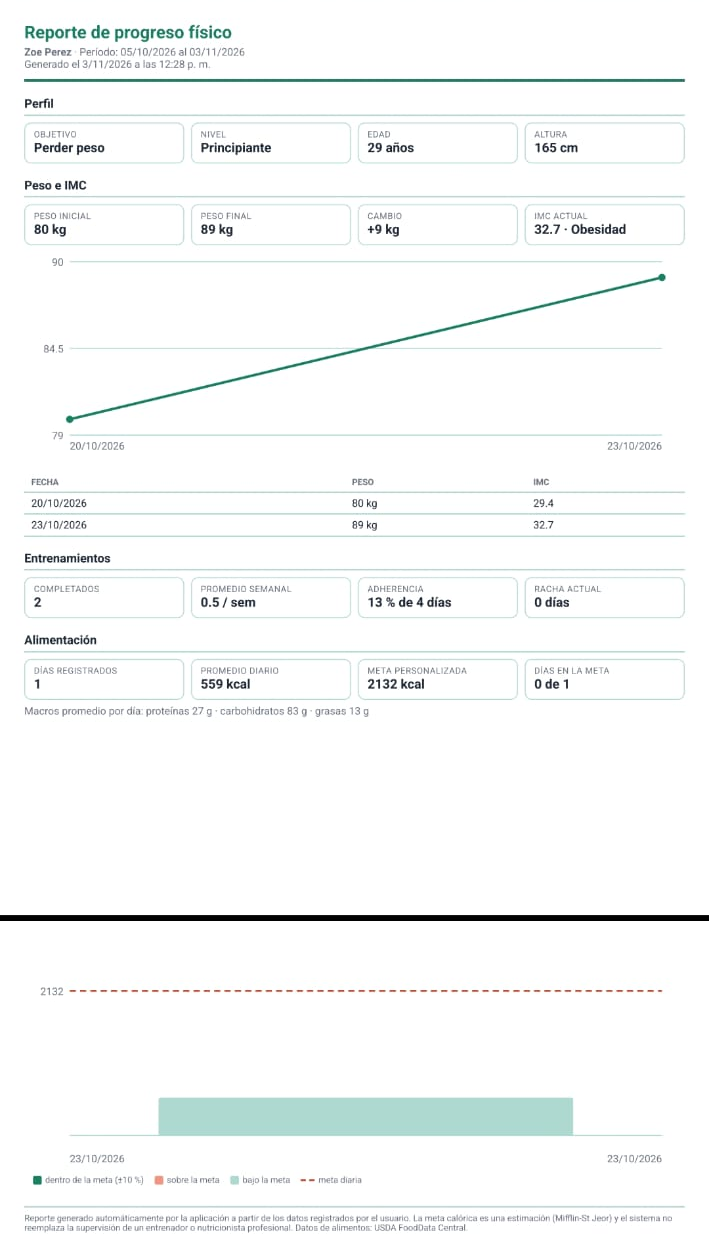
\includegraphics[height=0.36\textheight,keepaspectratio]{figuras/reporte-progreso-pdf.png}}
    \caption{Reporte de progreso físico en PDF generado en el dispositivo de prueba}
    \label{fig:reporte-pdf}
    \fuente{Elaboración propia. Captura de pantalla del reporte generado por la
    aplicación en el Infinix HOT 50 Pro+ (3 de noviembre de 2026).}
\end{figure}

A continuación, se describe la \emph{Story Card} del reporte de progreso en PDF:

\begin{table}[H]
\centering
\small
\renewcommand{\arraystretch}{1.2}

\begin{tabularx}{\textwidth}{|Y|Y|Y|}
\hline
\rowcolor{encabezado}
\textbf{Story Card} & \textbf{Nombre del proyecto} & \textbf{Estimación} \\
\hline
13 & CoachApp & Por completar \\
\hline

\multicolumn{2}{|l|}{\textbf{Nombre.} Reporte de progreso en PDF}
& \textbf{Fecha.} Por completar \\
\hline

\multicolumn{3}{|l|}{\textbf{Descripción}} \\
\hline
\multicolumn{3}{|p{\dimexpr\textwidth-2\tabcolsep-2\arrayrulewidth\relax}|}{%
El usuario genera un reporte de su progreso en PDF para guardarlo o
compartirlo.
} \\
\hline

\multicolumn{3}{|l|}{\textbf{Prueba de aceptación}} \\
\hline

\multicolumn{3}{|p{\dimexpr\textwidth-2\tabcolsep-2\arrayrulewidth\relax}|}{%
Generar el reporte eligiendo el período (7, 30, 90 días o todo el historial) y
comprobar que el PDF incluye perfil, peso e IMC, entrenamientos y
alimentación, y que se abre la hoja de compartir del sistema.
} \\
\hline

\multicolumn{2}{|l|}{\textbf{Excepciones}}
& \textbf{Riesgo.} Por evaluar \\
\hline

\multicolumn{3}{|p{\dimexpr\textwidth-2\tabcolsep-2\arrayrulewidth\relax}|}{%
Sin excepciones definidas.
} \\
\hline

\end{tabularx}
\caption{Story Card 13: Reporte de progreso en PDF}
\label{tab:hu-it6-reporte}
\fuente{Elaboración propia.}
\end{table}

\subsubsection{Pantalla de inicio}

En esta pantalla se puede observar la pantalla principal de la aplicación, que
saluda al usuario por su nombre. La tarjeta \emph{Hoy} presenta el día de la
rutina activa con su enfoque y el número de ejercicios, junto con los botones
para empezar el día y ver sus detalles. La sección \emph{Esta semana} muestra
la racha y los días completados de la semana, y el acceso \emph{Escanear
máquina} abre el escáner para identificar una máquina con la cámara
(Figura~\ref{fig:cap-inicio}).

\captura{inicio}{Pantalla de inicio}{fig:cap-inicio}

A continuación, se describe la \emph{Story Card} de la pantalla de inicio:

\begin{table}[H]
\centering
\small
\renewcommand{\arraystretch}{1.2}

\begin{tabularx}{\textwidth}{|Y|Y|Y|}
\hline
\rowcolor{encabezado}
\textbf{Story Card} & \textbf{Nombre del proyecto} & \textbf{Estimación} \\
\hline
14 & CoachApp & Por completar \\
\hline

\multicolumn{2}{|l|}{\textbf{Nombre.} Pantalla de inicio}
& \textbf{Fecha.} Por completar \\
\hline

\multicolumn{3}{|l|}{\textbf{Descripción}} \\
\hline
\multicolumn{3}{|p{\dimexpr\textwidth-2\tabcolsep-2\arrayrulewidth\relax}|}{%
El usuario ve en el inicio un resumen de su rutina activa y de sus registros.
} \\
\hline

\multicolumn{3}{|l|}{\textbf{Prueba de aceptación}} \\
\hline

\multicolumn{3}{|p{\dimexpr\textwidth-2\tabcolsep-2\arrayrulewidth\relax}|}{%
Abrir el inicio y comprobar que muestra la rutina activa, su número de
ejercicios y días por semana, y el número real de registros de peso.
} \\
\hline

\multicolumn{2}{|l|}{\textbf{Excepciones}}
& \textbf{Riesgo.} Por evaluar \\
\hline

\multicolumn{3}{|p{\dimexpr\textwidth-2\tabcolsep-2\arrayrulewidth\relax}|}{%
Sin excepciones definidas.
} \\
\hline

\end{tabularx}
\caption{Story Card 14: Pantalla de inicio}
\label{tab:hu-it6-inicio}
\fuente{Elaboración propia.}
\end{table}

\subsubsection{Codificación}

\paragraph{Registro del progreso.} \archivo{ProgressController} valida el
peso (entre 10 y 500~kg), la estatura opcional y unas notas de hasta 500
caracteres; si hay estatura, calcula el IMC reutilizando
\archivo{bmiCalculator}, y guarda el registro en
\archivo{usuarios/\{uid\}/progresoFisico}. Para evitar que el usuario
reescriba su estatura, la pantalla la precarga desde el perfil.

\paragraph{Visualización del progreso.} La vista \emph{Cuerpo} presenta los
últimos ocho registros en un gráfico de peso o IMC, la variación respecto al
primer registro, la categoría de IMC actual y el historial de mediciones.
Estos indicadores se calculan a partir de los registros observados en tiempo
real, sin crear una colección adicional de reportes.

\paragraph{Reporte personalizado en PDF.} El usuario puede generar un reporte
de 7, 30 o 90 días, o de todo su historial. \archivo{ReportsController}
reúne los datos; \archivo{progressReport.ts} calcula el resumen y construye
el HTML; y \archivo{pdfService.ts} genera y comparte el PDF mediante
\archivo{expo-print} y \archivo{expo-sharing}. El documento incluye perfil,
peso e IMC, entrenamientos y alimentación
(Figura~\ref{fig:reporte-pdf}). La comprobación en el dispositivo de prueba se
documenta en la sección~\ref{sec:des-pruebas}.

\paragraph{Seguimiento de entrenamientos.} El usuario marca los días
completados de su rutina. \archivo{WorkoutsController} registra cada
entrenamiento con la fecha local como identificador, lo que evita duplicar
el registro del mismo día. A partir de esas fechas se calculan la racha,
los días entrenados en la semana y el total acumulado. La racha se cuenta
desde ayer si el entrenamiento de hoy aún no se ha completado, para mantenerla
vigente durante el día (Código~\ref{lst:racha}).

\begin{lstlisting}[language=TypeScript, caption={Cálculo de la racha de entrenamientos}, label={lst:racha}]
export function calcularRacha(
  fechasCompletadas: ReadonlySet<string>, ahora: Date,
): number {
  const cursor = inicioDelDia(ahora);
  // Si hoy aun no se completo, la racha se evalua desde ayer.
  if (!fechasCompletadas.has(formatearFechaISO(cursor))) {
    cursor.setDate(cursor.getDate() - 1);
  }
  let racha = 0;
  while (fechasCompletadas.has(formatearFechaISO(cursor))) {
    racha++;
    cursor.setDate(cursor.getDate() - 1);
  }
  return racha;
}
\end{lstlisting}

